\documentclass{article}
\usepackage{geometry}
\usepackage{fancyhdr}
\usepackage{amsmath ,amsthm ,amssymb}
\usepackage{graphicx}
\usepackage{hyperref}

% Eigene Makros
\DeclareMathOperator{\diag}{\mathrm{diag}}
\newcommand{\partiell}[3][]{\frac{\partial^{#1}#2}{\partial{#3}^{#1}}}
\newcommand{\diff}[3][]{\frac{\mathrm{d}^{#1}#2}{\mathrm{d}{#3}^{#1}}}
\newcommand{\dr}{\mathrm{d}}
\newcommand{\vect}[1]{\boldsymbol #1}
\newcommand{\Reals}{\mathds R}
\newcommand{\Compl}{\mathds C}
\DeclareMathOperator{\Real}{\mathfrak R}
\DeclareMathOperator{\Imag}{\mathfrak I}
\newcommand{\norm}[1]{\left\|#1\right\|}
\newcommand{\abs}[1]{\left|#1\right|}
\newcommand{\skalprod}[2]{\langle#1,#2\rangle}
\DeclareMathOperator{\grad}{\mathrm{grad}}
\renewcommand{\div}{\mathrm{div}}

\title{Oberseminar Regelungstechnik \\ Regler- und Kalmanfilterentwurf für einen Helikopterversuchstand}
\author{Tilo Stock, Clemens Bilsing, Robert Heedt}
\date {23.11.2018}
\begin{document}
	\maketitle
	\tableofcontents
	\newpage
	\section{Modellbildung}
	Zur Modellbildung des Systems wurde der Lagrange-Formalismus zweiter Art angewendet. Für Systeme mit generalisiertem Potential lautet die Lagrange Gleichung 
	\begin{equation}
	L = T -V
	\end{equation}
	wobei $T$ jeweils die kinetische und $V$ die potentielle Energie des System bezeichnen.
	Mit der Betrachtung von nicht-konservativen Kräften $Q_i$ ergibt sich die Lagrange-Funktion
	\begin{equation}\label{eq:lagrange}
	\diff{}{t} \partiell{L}{\dot{q_i}} - \partiell{L}{q_i}=Q_i
	\end{equation}
	Wobei das Koordinatensystem des Modells $q_i$ festgelegt wurde als
	\begin{equation}
	q = \begin{pmatrix}
	p\\e\\\lambda
	\end{pmatrix}
	\end{equation}
	\subsection{Bestimmung der kinetischen- und potentiellen Energien}
	Zur Bestimmung der kinetischen Energie $T$ wurde die Rotation jeder einzelnen Masse um jede Koordinatenachse betrachtet und aufsummiert.
	\begin{equation}
	\begin{split}
	T&= m_p l_p^2\dot{p}^2 + \frac{1}{2}m_cl_c^2\dot{e}^2 
	+ m_p(l_h^2+(l_p\sin p)^2)\dot{e}^2\\
	&+ \frac{1}{2} m_c (l_c \cos e)^2\dot{\lambda}^2\\
	&+ \frac{1}{2} m_p((l_h \cos e +l_p \sin p \sin e)^2+(l_p \cos p)^2)\dot{\lambda}^2\\
	&+ \frac{1}{2} m_p((l_h \cos e -l_p \sin p \sin e)^2+(l_p \cos p)^2)\dot{\lambda}^2
	\end{split}
	\end{equation}
	Was vereinfacht werden kann zu
	\begin{equation}
	\begin{split}
	T&= m_p l_p^2\dot{p}^2 + \frac{1}{2}m_cl_c^2\dot{e}^2 
	+ m_p(l_h^2+(l_p\sin p)^2)\dot{e}^2\\
	&+ \frac{1}{2} m_c (l_c \cos e)^2\dot{\lambda}^2\\
	&+ m_p((l_h \cos e)^2 + (l_p \sin p \sin e)^2+(l_p \cos p)^2)\dot{\lambda}^2
	\end{split}
	\end{equation}
	Die potentielle Energie $V$ lautet
	\begin{equation}
	V = -m_c l_c g \sin e + 2 m_p l_h g \sin e
	\end{equation}
	Wodurch sich die Lagrange Funktion $L$ ergibt zu 
	\begin{equation}
	\begin{split}
	L = T - V&= m_p l_p^2\dot{p}^2 + \frac{1}{2}m_cl_c^2\dot{e}^2 
	+ m_p(l_h^2+(l_p\sin p)^2)\dot{e}^2\\
	&+ \frac{1}{2} m_c (l_c \cos e)^2\dot{\lambda}^2\\
	&+ m_p((l_h \cos e)^2 + (l_p \sin p \sin e)^2+(l_p \cos p)^2)\dot{\lambda}^2\\
	&+ m_c l_c g \sin e - 2 m_p l_h g \sin e
	\end{split}
	\end{equation}
	\subsection{Bestimmung der nicht-konservativen Kräfte}
	Die durch die Rotation der Rotoren entstehen nicht-konservative Kräfte, welche wie folgt vereinfacht\footnote{Die Darstellung von $Q_e$ und $Q_\lambda$ ist vereinfacht worden, damit $(F_f + F_b)$ ausgeklammert werden konnte.} dargestellt werden können:
	\begin{align}
	Q_p &= (F_f - F_b)l_p\\
	Q_e &= (F_f + F_b)l_h  \cos p\\
	Q_\lambda &= (F_f + F_b)l_h \cos e \sin p
	\end{align}
	\subsection{Aufstellen der Bewegungsgleichung um $p$}
	\begin{align}
	\partiell{L}{\dot{p}} &= 2m_p l_p^2 \dot{p}\\
	\diff{}{t} \partiell{L}{\dot{p}} &= 2m_p l_p^2 \ddot{p}
	\end{align}
	\begin{equation}
	\begin{split}
	\partiell{L}{p} &= \partiell{}{p} (m_p l_p^2 \dot{e}^2 \sin^2 (p) 
	+ m_p l_p^2 \sin^2 (e) \dot{\lambda}^2 \sin^2 (p)
	+ m_p l_p^2 \dot{\lambda}^2 \cos^2 p)\\
	&= 2 m_p l_p^2 \dot{e}^2 \cos p \sin p + 2 m_p l_p^2 \sin^2 (e) \dot{\lambda}^2 \cos p \sin p 
	- 2 m_p l_p^2 \dot{\lambda}^2 \cos p \sin p\\
	&= 2 m_p l_p^2 \cos p \sin p (\dot{e}^2+ \sin^2 (e) \dot{\lambda}^2- \dot{\lambda}^2)\\
	&= 2 m_p l_p^2 \cos p \sin p (\dot{e}^2- \cos^2 (e) \dot{\lambda}^2)
	\end{split}
	\end{equation}
	Eingesetzt in \eqref{eq:lagrange} ergibt:
	\begin{equation}
	\underbrace{2m_p l_p^2}_{J_p} \ddot{p} -  \underbrace{2 m_p l_p^2}_{J_p} \cos (p) \sin (p) (\dot{e}^2- \cos^2 (e) \dot{\lambda}^2) = (F_f - F_b)l_p = V_d \underbrace{K_f l_p}_{L_1}
	\end{equation}
	\subsection{Aufstellen der Bewegungsgleichung um $e$}
	\begin{equation}
	\partiell{L}{\dot{e}} = 2(\frac{1}{2}m_cl_c^2
	+ m_p(l_h^2+(l_p\sin p)^2))\dot{e}
	\end{equation}
	\begin{equation}
	\diff{}{t}\partiell{L}{\dot{e}} = (m_cl_c^2
	+ 2 m_p(l_h^2+l_p^2\sin^2 p))\ddot{e}
	\end{equation}
	\begin{equation}
	\begin{split}
	\partiell{L}{e} &= \partiell{}{e}(\frac{1}{2} m_c l_c^2 \dot{\lambda}^2 \cos^2 (e) + m_p \dot{\lambda}^2 (l_h^2 \cos^2 (e) + l_p^2 \sin^2 (p) \sin^2 (e))
	+ m_c l_c g \sin e - 2 m_p l_h g \sin e)\\
	&= -m_c l_c^2 \dot{\lambda}^2 \cos e \sin e + 2 m_p \dot{\lambda}^2 \cos e \sin e (-l_h^2  + l_p^2 \sin^2 (p) ) + g(m_c l_c - 2 m_p l_h) \cos e\\
	&= \cos e \sin e  (-m_c l_c^2 + 2 m_p (l_p^2 \sin^2 (p) -l_h^2  )) \dot{\lambda}^2+ g(m_c l_c - 2 m_p l_h) \cos e
	\end{split}
	\end{equation}
	Eingesetzt in \eqref{eq:lagrange} ergibt:
	\begin{equation}
	\begin{split}
	&(m_cl_c^2+ 2 m_p(l_h^2+l_p^2\sin^2 p))\ddot{e} - \cos e \sin e (-m_c l_c^2 + 2 m_p (l_p^2 \sin^2 (p) -l_h^2  ))\dot{\lambda}^2 \\
	& - g(m_c l_c - 2 m_p l_h) \cos e = (F_f + F_b)l_h  \cos p
	\end{split}
	\end{equation}
	
	\begin{equation}
	\begin{split}
	&\overbrace{(m_cl_c^2+ 2 m_p(l_h^2+l_p^2\sin^2 p))}^{J_e}\ddot{e} + \cos e \sin e \overbrace{(m_c l_c^2 + 2 m_p ( l_h^2 -l_p^2 \sin^2 (p) ))}^{\approx J_e} \dot{\lambda}^2 \\
	&= \underbrace{g(m_c l_c - 2 m_p l_h)}_{L_2} \cos e + V_s \underbrace{ K_f l_h}_{L_3}  \cos p
	\end{split}
	\end{equation}
	\begin{figure}[ht]
		\centering
		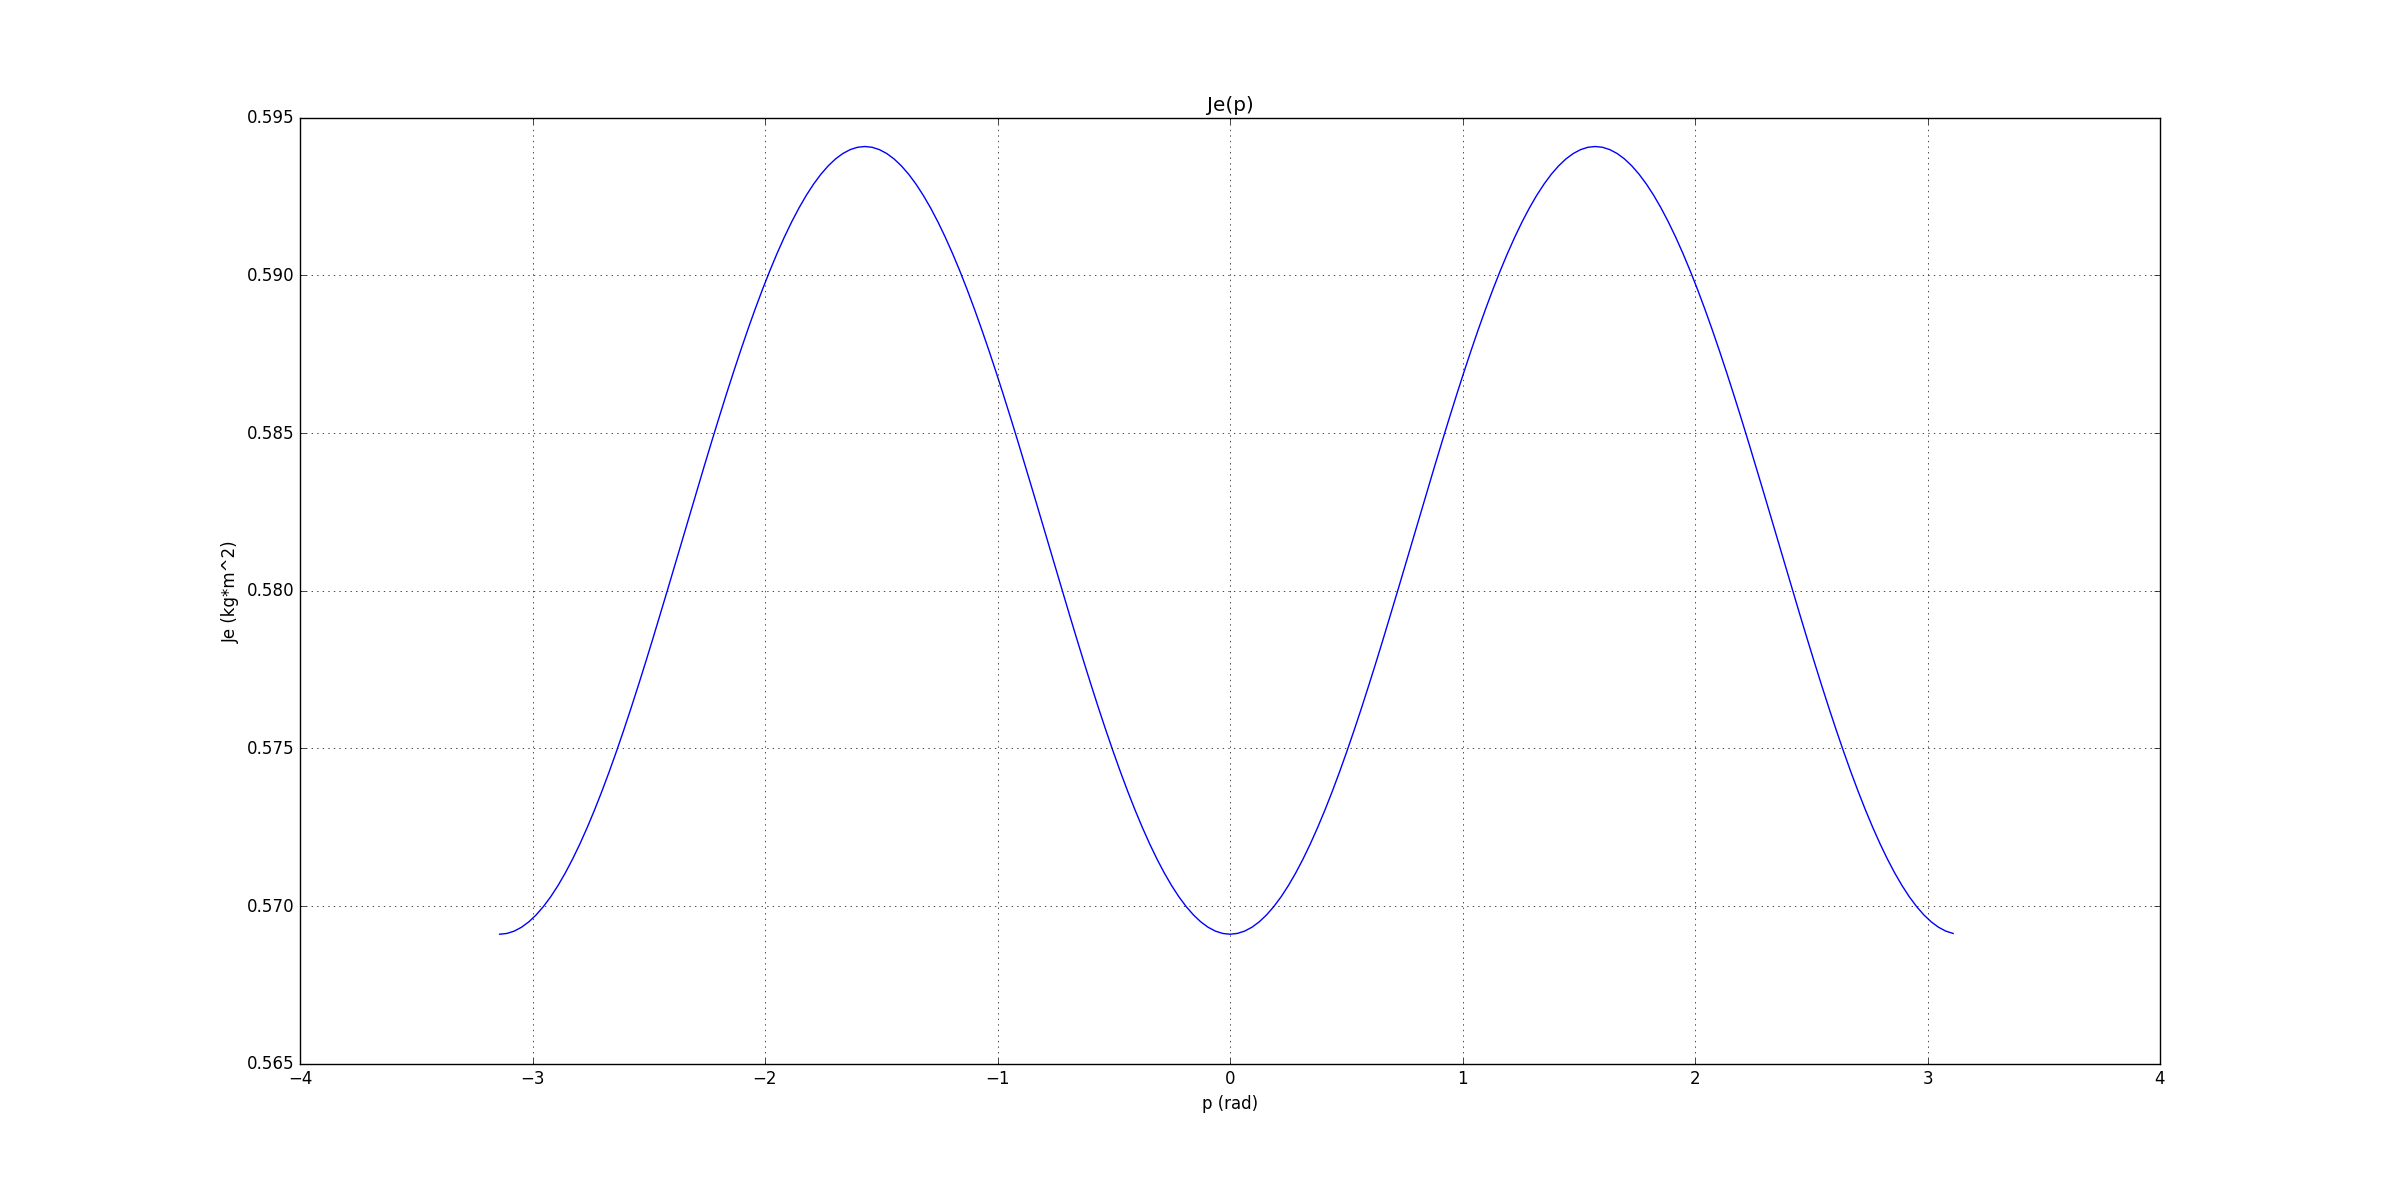
\includegraphics[width=1\textwidth]{images/J_e}
		\caption{$J_e$ in Abhängigkeit des Winkels $p$}
		\label{fig:J_e}
	\end{figure}
	\subsection{Aufstellen der Bewegungsgleichung um $\lambda$}
	\begin{equation}
	\partiell{L}{\dot{\lambda}} = (m_c (l_c \cos e)^2
	+ 2 m_p((l_h \cos e)^2 + (l_p \sin p \sin e)^2+(l_p \cos p)^2))\dot{\lambda}
	\end{equation}
	\begin{equation}
	\diff{}{t}\partiell{L}{\dot{\lambda}} = (m_c (l_c \cos e)^2
	+ 2 m_p((l_h \cos e)^2 + (l_p \sin p \sin e)^2+(l_p \cos p)^2))\ddot{\lambda}
	\end{equation}
	\begin{equation}
	\partiell{L}{\lambda} = 0
	\end{equation}
	Eingesetzt in \eqref{eq:lagrange} ergibt:
	\begin{equation}
	\underbrace{(m_c (l_c \cos e)^2
	+ 2 m_p((l_h \cos e)^2 + (l_p \sin p \sin e)^2+(l_p \cos p)^2))}_{J_\lambda}\ddot{\lambda} =  V_s \underbrace{K_f l_h}_{L_4} \cos e \sin p
	\end{equation}
	\begin{figure}[ht]
		\centering
		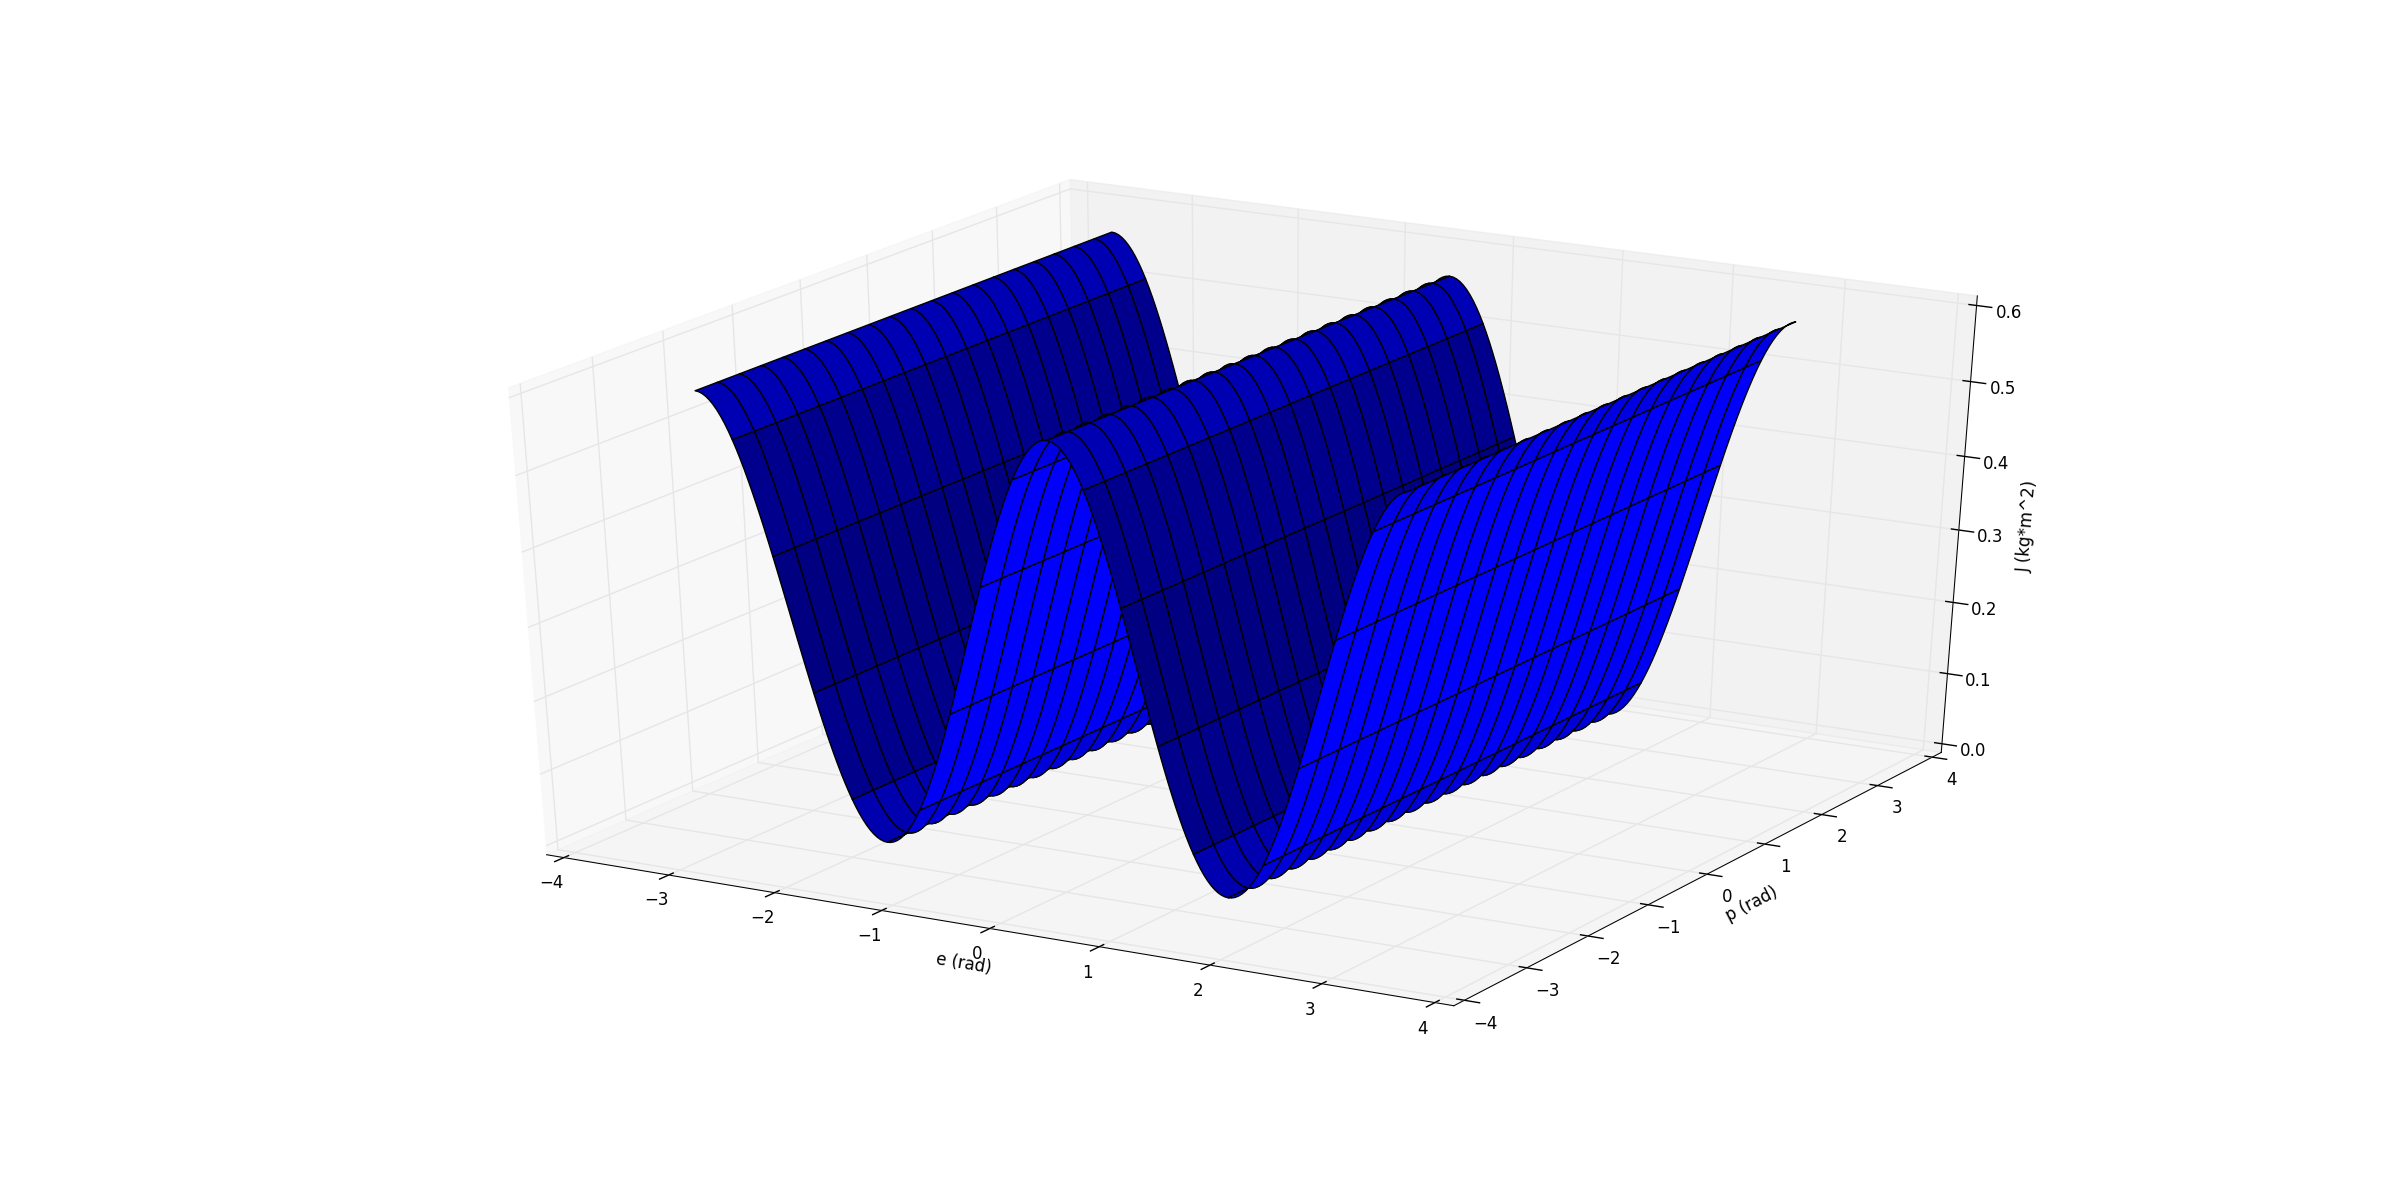
\includegraphics[width=1\textwidth]{images/J_l}
		\caption{$J_\lambda$ in Abhängigkeit der Winkel $p$ und $e$}
		\label{fig:J_l}
	\end{figure}	
	\subsection{Zusammenfassen der Bewegungsgleichungen}
	Insgesamt kann das System mit wenigen Vereinfachungen und ohne Berücksichtigung von Reibung wie folgt dargestellt werden:
	\begin{align}
	J_p \ddot{p} - J_p \cos (p) \sin (p) (\dot{e}^2- \cos^2 (e) \dot{\lambda}^2) &= V_d L_1\\
	J_e\ddot{e} + J_e \cos (e) \sin (e) \dot{\lambda}^2 
	&= L_2 \cos e + V_s L_3 \cos p\\
	J_\lambda \ddot{\lambda} &= V_s L_4 \cos e \sin p
	\end{align}
	\subsection{Erweiterung der Bewegungsgleichungen mit Gleitreibung}
	Durch Hinzufügen von Gleitreibung kommt ein zusätzliches Drehmoment in Abhängigkeit der jeweiligen Winkelgeschwindigkeit $\dot{q_i}$ und des Reibkoeffizienten $\mu_i$  hinzu.
	\begin{align}
	J_p \ddot{p} + \mu_p \dot{p} - J_p \cos (p) \sin (p) (\dot{e}^2- \cos^2 (e) \dot{\lambda}^2) &= V_d L_1\\
	J_e\ddot{e} + \mu_e \dot{e} + J_e \cos (e) \sin (e) \dot{\lambda}^2 
	&= L_2 \cos e + V_s L_3 \cos p\\
	J_\lambda \ddot{\lambda} + \mu_\lambda \dot{\lambda} &= V_s L_4 \cos e \sin p
	\end{align}
	\subsection{Erweiterung des Systems durch Rotordrehzahlen}
	Die Kraft jedes Rotors resultiert nun aus der Drehzahl jedes Motors, wobei diese durch einen Tiefpass 1. Ordnung beschrieben werden können.
	\begin{align}
	T_f \dot{f} + f &= K_f V_f\\
	T_b \dot{b} + b &= K_b V_b
	\end{align}
	Dabei beschreibt $f$ und $b$ die Drehzahl der beiden Motoren und $T_f$ sowie $T_b$ deren Zeitkonstante.
	Damit kann die auf das System resultierende Kraft beschrieben werden durch:
	\begin{equation}
	F_s = F_f + F_b = K (f + b)
	\end{equation}
	\begin{equation}
	F_b = F_f - F_b = K (f - b)
	\end{equation}
	Weiterhin entstehen aus der Rotordrehzahl das jeweiliges Drehmoment $M_f$ und $M_b$ der Elektromotoren. Diese bewirken ein zusätzliches Moment auf die Drehachse um $e$ und $\lambda$.
	\begin{align}
	M_{M,e} &= \sin (p) (M_f - M_b) =\sin (p) K_M (f-b) \\
	M_{M,\lambda} &= \cos (e) \cos (p) (M_b - M_f) =\cos (e) \cos (p) K_M (b-f)
	\end{align}
	Das resultierende System ist daher:
	\begin{align}
	&J_p \ddot{p} + \mu_p \dot{p} - J_p \cos (p) \sin (p) (\dot{e}^2- \cos^2 (e) \dot{\lambda}^2) = K l_p (f - b)\\
	&J_e\ddot{e} + \mu_e \dot{e} + J_e \cos (e) \sin (e) \dot{\lambda}^2 
	= L_2 \cos e + K l_h \cos p (f + b) + \sin (p) K_M (f-b)\\
	&J_\lambda \ddot{\lambda} + \mu_\lambda \dot{\lambda} = K l_h \cos e \sin p (f + b) +\cos (e) \cos (p) K_M (b-f)
	\end{align}
	
\end{document}